\documentclass[12pt]{article}
\usepackage[T1]{fontenc}
\usepackage[latin1]{inputenc}
\usepackage[italian]{babel}
\usepackage{latexsym}
\usepackage{epsfig}
\usepackage{fancybox}
\usepackage{rotating}
\usepackage{graphicx}

\textwidth 15.5cm
\textheight 22.5cm
\topmargin 0cm
\evensidemargin 0in
\oddsidemargin 0in


\def\bbbr{{\rm I\!R}}
\def\bbbm{{\rm I\!M}}
\def\bbbn{{\rm I\!N}}

\def\sm{\setminus}
\newcommand {\ol}[1]{\overline{#1}}



\def\La{{\cal \Leftarrow}}
\def\Ra{{\cal \Rightarrow}}


\newtheorem{Teo}{Theorem}[section]
\newtheorem{Con}[Teo]{Conjecture}
\newtheorem{Que}{Question}
\newtheorem{Cor}[Teo]{Corollary}
\newtheorem{Property}[Teo]{Property}
\newtheorem{Pro}[Teo]{Proposition}
\newtheorem{Cla}[Teo]{Claim}
\newtheorem{Lem}[Teo]{Lemma}
\newtheorem{Def}{Teorema}
\newtheorem{Obs}[Teo]{Observation}
\newtheorem{Note}{Note}

\pagestyle{empty}
 
\begin{document}
\title{\textbf {Grafi}}
\author{}
\date{}
\maketitle
Queste note teoriche vogliono essere un supporto alle lezioni del Prof. Rizzi; quindi per facilitare la comprensione dei concetti teorici spiegati di seguito consideriamo come esempio il Problema 6 dell'esame del 28/09/2016; il mio consiglio � di leggere queste note seguendo parallelamente lo svolgimento del problema citato.  
\section{Planarit�}
Una delle prime richieste � quella di certificare se il grafo dato sia planare o meno. Per prima cosa cominciamo col definire il concetto di planarit�: un grafo � \emph{planare} se lo si pu� disegnare nel piano senza che nessuno dei suoi archi si incroci. 

\begin{figure}
\centering
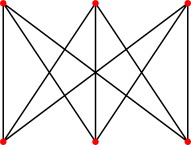
\includegraphics[width=0.30\textwidth]{K3,3.png} \quad 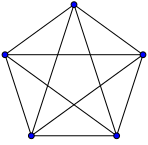
\includegraphics[width=0.30\textwidth]{K5.png}
\caption{$K_{3,3}$ a sinistra, $K_5$ a destra}
\end{figure}

Pertanto una volta che avrete \emph{intuito} se il grafo dato � planare o no, bisogna fornirne il relativo certificato e vi si possono presentare due casi:

\begin{itemize}
\item Se il grafo � \textbf{planare} allora il relativo certificato consiste solo nel disegnare il grafo \emph{planarizzato}(ovvero disegnarlo senza incrociare gli archi).\\
\item Se il grafo \textbf{non � planare} bisogna individuare o un $K_{3,3}$ o un $K_5$ \footnote{mostrati in figura 1} al suo interno. Questo pu� risultare pi� complicato. Si consideri il caso in cui si voglia individuare un $K_{3,3}$: � necessario selezionare tre nodi 'maschi' (colorateli di blu) e tre nodi 'femmine' (colorateli di rosso) e mostrare che da ogni nodo blu si raggiungono tutti e tre i nodi rossi. \emph{Non} � strettamente necessario che vi sia un solo arco che collega il primo nodo maschio a ciascuna femmina, ma � importante che tutti e sei i differenti percorsi non condividano nessun nodo e quindi nessun arco in comune. 
\end{itemize}


\section{Albero di peso minimo}
L'\emph{albero di peso minimo} � un albero contenente tutti i nodi del grafo, ma solo un sottoinsieme dei suoi archi, ovvero solo quelli necessari per collegare i nodi con un solo cammino \footnote{Definiamo \textbf{cammino} di un grafo G una sequenza di nodi $u_0, u_1, \dots, u_k$ tali che $(u_i, u_{i+1}) \in A$, per $i = 0,1,2, \dots, k-1$ e per A insieme di tutti gli archi di G.}. .\\

Il principale problema in questo esercizio � determinare se alcuni archi del grafo appartengano/ possano appartenere/ non appartengano alla soluzione ottima. A tal proposito possono essere utili alcune definizioni:
\begin{Def}
Definiamo \textbf{cammino semplice} un cammino in cui non ci sono nodi ripetuti, ovvero $u_i \ne u_j$ per $0 \le i < j \le k$; mentre se $u_0 = u_k$ allora il cammino � detto \textbf{chiuso}.
\end{Def}  
\begin{Def}
Un cammino sia semplice che chiuso, dove l'unica ripetizione � $u_0 = u_k$, � detto \textbf{ciclo}.
\end{Def}
\begin{Def}
Un \textbf{taglio} $C = (S,T)$ � la partizione dei vertici V di un grafo $G = (V,E)$ in due sottoinsiemi disgiunti S e T. Definiamo, inoltre, \textbf{insieme di taglio} di un taglio $C = (S,T)$ l'insieme $\{ (u,v) \in E | u \in S, v \in T \}$ degli archi che hanno un estremo in S e l'altro in T. 
\end{Def}
Data un infarinazione teorica, possiamo passare alla pratica. Anzitutto quello che dovete scolpirvi nella testa � che \emph{se non fornite il certificato, non ottenete punti}, quindi vediamo cos'� il certificato in questa tipologia di problemi. Per aiutarvi a comprendere, si pu� usare la seguente schematizzazione:
\begin{itemize}
\item Se l'arco considerato \textbf{appartiene} a tutte le soluzioni ottime, allora � necessario fornire un certificato di \textbf{taglio}, ovvero mostrare che l'arco considerato � di peso minimo tra gli archi che se eliminati separano un ristretto numero di nodi da tutti gli altri.\\ 
\item Se l'arco \textbf{non appartiene} a nessuna soluzione ottima, bisogna fornire un certificato di \textbf{ciclo}, ovvero bisogna trovare un ciclo in cui tale arco � di peso massimo.\\
\item Se l'arco \textbf{pu� appartenere} alle soluzioni ottime, allora bisogna addurre sia un certificato di \textbf{taglio} (in cui tale arco � di peso minimo), che di \textbf{ciclo} (dove invece � di peso massimo).
\end{itemize}

\section{Cammini minimi}
Il problema dei \emph{cammini minimi} pu� essere espresso come segue: dato un grafo $G = (N, A)$, con pesi interi relativi agli archi in A, e dato un nodo $r \in N$, trovare un cammino da r a u, per ogni nodo $u \in N$, tale che la somma delle lunghezze degli archi nel cammino sia la pi� piccola possibile, ovvero bisogna trovare quel cammino che collega due vertici r e u, che minimizza la somma dei costi associati all'attraversamento di ogni arco. Al fine di ottenere la soluzione ammissibile � necessario che ogni nodo sia raggiungibile da r con un cammino. Pertanto il grafo G non deve contenere cicli di lunghezza negativa o archi di peso negativo, infatti in tal caso si otterrebbero che la lunghezza minima di un qualsiasi cammino un nodo di un ciclo negativo non sarebbe uniformemente limitata.\\
Si osservi che due cammini distinti possono avere un tratto iniziale in comune, da r fino ad un certo nodo s, e poi divergere verso le rispettive destinazioni u e v, ma al contrario non possono convergere ad un nodo comune s dopo aver percorso due tratti iniziali distinti, perch� se cos� fosse ci sarebbero due cammini distinti da r a s, mentre si richiede l'unicit�. Possiamo quindi definire \emph{soluzione ammissibile} un albero di copertura\footnote{per \textbf{albero di copertura} si intende un albero che contiene tutti nodi del grafo ma solo un sottoinsieme di archi, solo quelli necessari per connettere tutti i nodi del grafo}, radicato in r, che include il cammino da r ad ogni altro nodo.\\

Sebbene sia confortante sapere quando una soluzione � ammissibile, si vuole cercare la \emph{soluzione ottima}. Consideriamo la seguente notazione: ogni nodo \emph{i} del grafo $G = (N, A)$ � caratterizzato da un intero $d_i$ che indica la distanza i da r in T, soluzione ammissibile, e che � pari alle lunghezze degli archi ($c_{ij}$) che si trovano nell'unico cammino tra r ed i in T. Forniamo quindi il seguente risultato:
\begin{Teo}[Bellman]
Una soluzione ammissibile T � ottima se e solo se valgono le seguenti condizioni: $d_i + c_{ij} = d_j$ per ogni arco $(i,j) \in T$, e $d_i + c_{ij} \ge d_j$ per ogni arco $(i,j) \in A$.
\end{Teo}   
Tale risultato � fondamentale per caratterizzare una soluzione che sia ottima e per creare un algoritmo che identifichi tale soluzione. Uno degli algoritmi pi� usati a tal scopo � quello di Dijkstra, che si articola come segue: 
\begin{itemize}
\item Ogni nodo all'inizio ha valore $\infty$ tranne quello di partenza che ha valore 0.\\
\item Ogni volta di sceglie il nodo con potenziale minore e lo si rende definitivo e non pu� pi� essere riaggiornato, dove per potenziale si intende la somma del valore del nodo precedente e del costo del collegamento. I potenziali definitivi indicano la distanza di quel nodo da quello di partenza.\\
\item Dopo aver aggiornato il potenziale di un nodo si ricomincia la procedura.
\end{itemize}
In questo modo abbiamo ottenuto un albero di cammino minimo da un nodo di partenza s ad uno di arrivo t. 
%%%%%%%%%%%%%%%%%%%%%%%%%%%%%%%

\end{document}